\section[Conditions]{\textbf{Case Conditions}}

\begin{frame}{\small Geometry and Aerodynamic Conditions}
\scriptsize
\begin{columns}[T,onlytextwidth]

%------------------------------------------------
\begin{column}{0.46\textwidth}

\begin{figure}
    \centering
    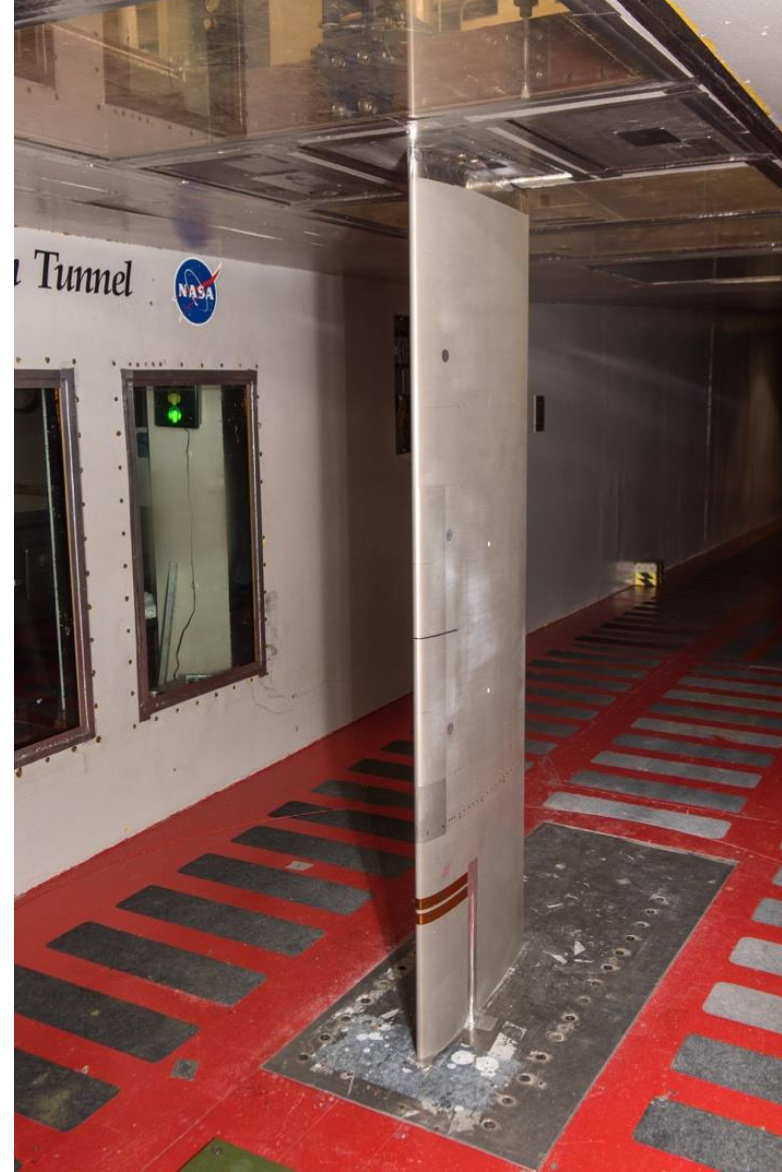
\includegraphics[height=0.66\textheight]{FIGURES_CONDITIONS/NACA0012_TUNNEL_VIEW.png}
\end{figure}

\end{column}

%------------------------------------------------
\begin{column}{0.50\textwidth}

\textbf{NASA Icing Research Tunnel}

\vspace{0.25cm}

\begin{tabular}{ll}
Airfoil                  & NACA0012 \\
Chord, $c$               & $0.5334~\mathrm{m}$ \\
Angle of attack          & $4^\circ$ \\
\end{tabular}

\vspace{0.5cm}

\textbf{Aerodynamic Conditions}

\vspace{0.2cm}

\begin{tabular}{ll}
$M_\infty$               & $0.3114$ \\
$U_\infty$               & $102.15~\mathrm{m/s}$ \\
$T_\infty$               & $267.75~\mathrm{K}$ \\
$\rho_\infty$            & $1.1884~\mathrm{kg/m^3}$ \\
$Re_c$                   & $3.8441\times10^6$ \\
\end{tabular}

\vspace{0.5cm}

\textbf{Quantities of Interest}

\vspace{0.15cm}

\[
C_L,\qquad C_D,\qquad C_M,\qquad C_p
\]

\end{column}

\end{columns}

\end{frame}

\begin{frame}[shrink]{\small Icing Conditions}
\scriptsize
\begin{columns}[T,onlytextwidth]

%------------------------------------------------
\begin{column}{0.43\textwidth}

\begin{figure}
    \centering
    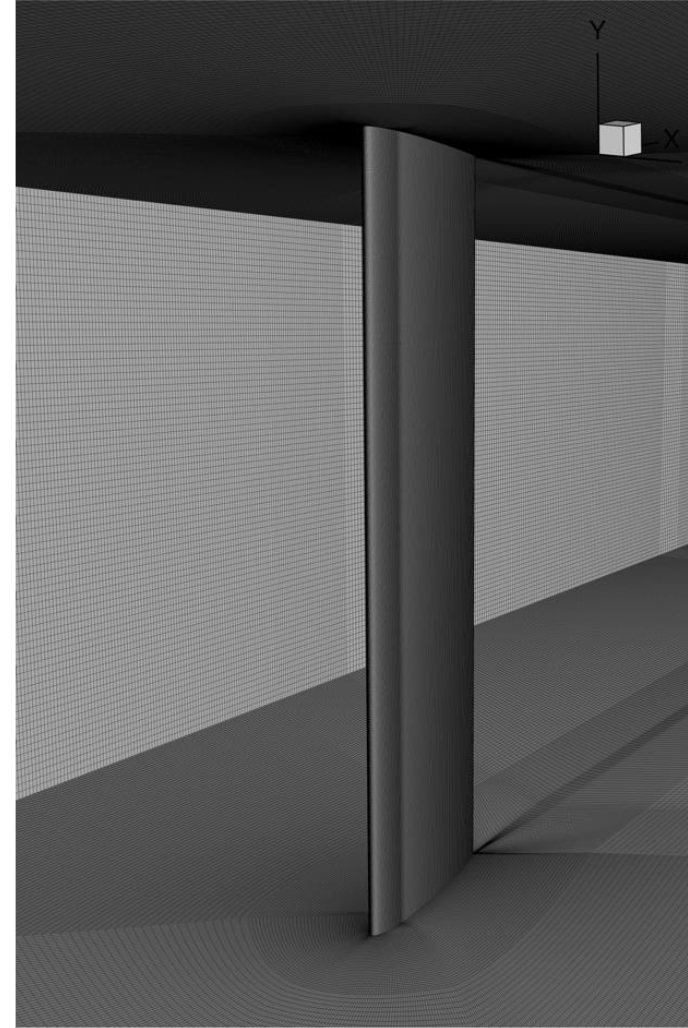
\includegraphics[height=0.56\textheight]{FIGURES_CONDITIONS/NACA0012_MESH_VIEW.png}
\end{figure}

\vspace{-0.25cm}

\centering
\begin{tabular}{lcc}
\toprule
\textbf{Grid} & \textbf{Nodes} & \textbf{Elements} \\
\midrule
L1 & $60.45$ M & $59.86$ M \\
L2 & $27.31$ M & $26.99$ M \\
L3 & $11.23$ M & $11.08$ M \\
L4 & $5.95$ M  & $5.86$ M \\
\bottomrule
\end{tabular}

\end{column}

%------------------------------------------------
\begin{column}{0.53\textwidth}

\begin{tabular}{lcc}
\toprule
 & \textbf{AE3932} & \textbf{AE3933} \\
\midrule
$T_0$ [$^\circ$C]       & $-5.6$ & $-2.2$ \\
$T_\infty$ [K]          & $262.305$ & $265.8$ \\
$M_\infty$              & $0.3151$ & $0.3127$ \\
$U_\infty$ [m/s]        & $102.31$ & $102.19$ \\
LWC [g/m$^3$]           & $0.55$ & $0.55$ \\
MVD [$\mu$m]            & $20$ & $20$ \\
Exposure time [min]     & $7$ & $7$ \\
\midrule
\textbf{Exp. ice mass [g]} & \textbf{101.0} & \textbf{85.9} \\
\bottomrule
\end{tabular}

\begin{block}{\scriptsize Experimental Observation}

The warmer AE3933 condition produces approximately \textbf{15\% less ice mass} than AE3932
($85.9$ g vs.\ $101.0$ g). This difference will be revisited when assessing the predicted
thermodynamic mass balance and ice accretion.
\end{block}

\textbf{Droplet Distribution}

\begin{itemize}
    \item Single-bin to 15-bin distributions
    \item Total LWC preserved between distributions
    \item Evaluated across all four grid levels
\end{itemize}


\textbf{Quantities of Interest}
\vspace{-0.25cm}
\[
\beta,\quad HTC,\quad T_s,\quad f,\quad
m_{\mathrm{water}},\quad m_{\mathrm{ice}},\quad
m_{\mathrm{evap}}
\]

\end{column}

\end{columns}

\end{frame}
